% ============================================================================
% Spatial Context Causal Adjustment for Geographic Observational Studies
% ============================================================================
% Target journal: International Journal of Geographical Information Science
% ============================================================================
\documentclass{article}

\usepackage{amsmath,amssymb}
\usepackage{booktabs}
\usepackage{graphicx}
\usepackage{multirow}
\usepackage{caption}
\usepackage{subcaption}
\usepackage{algorithm}
\usepackage{algorithmic}
\usepackage{hyperref}
\usepackage{color}
\usepackage{natbib}
\usepackage{tikz}
\usetikzlibrary{positioning,arrows.meta,shapes.geometric,fit,calc}
\graphicspath{{./figures/}{./}}
\bibliographystyle{plainnat}
\newenvironment{keywords}{\par\noindent\textbf{Keywords:}\ }{\par}

\begin{document}

\title{\parbox{0.9\textwidth}{\centering Spatial Context Causal Adjustment\\for Geographic Observational Studies}}

\author{Ning Zhou$^{a}$ and Xiang Jing$^{a}$$^{\ast}$\thanks{$^\ast$Corresponding author. Email: jingxiang@pku.edu.cn}\\
$^{a}${\em School of Software and Microelectronics, Peking University, Beijing 100871, China}}

\date{}
\maketitle

\begin{abstract}
Geographic observational studies often estimate effects from data in which treatment assignment, outcomes, and unmeasured environmental conditions are spatially structured. Standard causal estimators can be applied to such data, but their credibility depends on whether the adjustment set captures relevant spatial context, whether treated and control units overlap after adjustment, and whether residual spatial structure remains after matching or weighting.

We introduce Spatial Context Causal Adjustment (SCCA), a reproducible workflow for constructing, diagnosing, and reporting spatial-context adjustment sets. SCCA treats coordinates, geometry, terrain, remote-sensing indices, land-cover descriptors, and learned geospatial embeddings as candidate context variables rather than as automatically valid controls. The workflow standardizes four steps: context feature construction, adjustment-set selection, common-support and covariate-balance diagnostics, and robustness checks including spatial block bootstrap, placebo exposure definitions, and residual spatial autocorrelation.

We evaluate SCCA using controlled multi-seed benchmarks and four real or historical case studies. In a Chongqing urban heat case with 5,000 sampled buildings, the full remote-sensing and terrain context specification estimated a modest positive effect of high-rise buildings on summer land surface temperature (ATT = 0.244$^\circ$C, 95\% CI [0.148, 0.346]) while achieving credible post-match balance (maximum standardized mean difference = 0.061). Historical cholera and county social-capital cases showed stable effect directions under ablation and bootstrap diagnostics, although two cholera cases retained bounded support because exposure-balance correlations remained high. A direct AlphaEarth embedding ablation did not improve balance over conventional remote-sensing and terrain variables in the Chongqing case.

These results support SCCA as a diagnostic method for making spatial causal adjustment more explicit and auditable. They do not establish that any single representation source, including geospatial foundation-model embeddings, is generally superior. The contribution is therefore a bounded method and evidence-grading protocol for geographic causal analysis rather than a claim of universal causal identification.
\end{abstract}

\begin{keywords}
spatial causal inference; spatial confounding; causal adjustment; propensity score matching; remote sensing; geospatial foundation models; robustness diagnostics
\end{keywords}


% ============================================================================
\section{Introduction}
\label{sec:intro}
% ============================================================================

Geographic information science increasingly supports policy questions that are causal rather than merely descriptive: whether urban form changes heat exposure, whether infrastructure changes disease risk, whether land-use interventions change environmental outcomes, or whether social context affects population health. These questions are usually studied from observational spatial data. Treatment is rarely randomized, spatial units are embedded in environmental gradients, and outcomes are measured at spatial resolutions that do not always match the intervention units.

The main difficulty is not the absence of causal estimators. Matching, weighting, regression adjustment, difference-in-differences, spatial panel models, and machine-learning estimators are all available to GIS researchers \citep{stuart2010matching, angrist2009mostly, athey2019estimating}. The difficulty is that spatial context determines both exposure and outcome. Elevation, slope, land cover, access, urban morphology, historical settlement, and administrative structure can all confound a geographic effect estimate. If these context variables are omitted, the estimate is vulnerable to spatial confounding. If they are added indiscriminately, the estimator may lose common support, amplify noise, or adjust for variables that are not valid confounders.

Recent geospatial representation methods make this problem more important. Remote-sensing indices and terrain variables are now easy to extract at scale, and geospatial foundation-model embeddings may encode broad environmental context \citep{brown2025alphaearth}. These representations are useful only if their role in causal adjustment is diagnosed. A dense embedding is not automatically a confounder, and a richer adjustment set is not automatically a better adjustment set. Geographic causal analysis therefore needs a workflow that asks a practical question: which spatial-context variables improve credible adjustment for this study, under visible diagnostics, and where does the evidence stop?

This paper proposes Spatial Context Causal Adjustment (SCCA). SCCA is a method workflow rather than a new estimator. It wraps standard estimators with spatial-context feature construction, adjustment-set comparison, common-support checks, post-adjustment balance diagnostics, spatial robustness tests, and an evidence grade. The central idea is deliberately conservative: spatial context is useful only when it improves a diagnosed adjustment design.

Our contributions are:

\begin{enumerate}
\item A formal SCCA workflow for representing, selecting, and diagnosing spatial-context adjustment sets in geographic observational studies.
\item A reproducible diagnostic protocol covering common support, covariate balance, spatial block bootstrap, placebo exposure definitions, residual spatial autocorrelation, and evidence grading.
\item Cross-case evidence from synthetic benchmarks, a Chongqing urban heat analysis, two historical cholera analyses, and a county social-capital validation case.
\item A bounded AlphaEarth embedding ablation showing that learned geospatial embeddings are a candidate context source but offered no clear diagnostic gain in the current Chongqing case.
\end{enumerate}

The paper is written around this bounded claim. We do not claim that SCCA eliminates unobserved spatial confounding, solves spatial interference, or proves that learned geospatial embeddings outperform conventional covariates. Instead, SCCA makes such claims harder to make without diagnostic evidence.


% ============================================================================
\section{Related Work}
\label{sec:related}
% ============================================================================

\subsection{Causal inference with spatial data}

Potential-outcome causal inference defines treatment effects by comparing outcomes under treatment and control states \citep{imbens2015causal}. In observational studies, the identifying assumption is conditional exchangeability: after adjustment for measured confounders, treatment assignment is as-if random. Matching and weighting operationalize this assumption by constructing comparable treated and control groups \citep{rosenbaum1983central, stuart2010matching}. In spatial studies, this assumption is difficult because geographic location and environment are themselves structured confounders.

Spatial econometrics and spatial statistics provide tools for autocorrelation, spillover, and spatial dependence \citep{anselin1988spatial}. These tools are essential, but they do not by themselves select valid adjustment sets. A spatial lag term can reduce residual autocorrelation while leaving treatment assignment confounded; a coordinate trend can absorb broad gradients while failing to represent local land-cover context. SCCA therefore treats spatial dependence diagnostics and causal adjustment diagnostics as related but distinct requirements.

\subsection{Spatial context as an adjustment source}

Geographic adjustment sets commonly include coordinates, administrative fixed effects, distance measures, terrain variables, land-cover classes, built-environment descriptors, and remote-sensing indices. These variables can proxy for otherwise unmeasured context. They can also create new problems if they are weakly related to treatment assignment, strongly collinear, measured at incompatible scales, or affected by the treatment itself. The SCCA workflow requires each candidate context source to pass common-support and balance checks before it is used to support a causal statement.

Learned geospatial embeddings extend this idea. Foundation-model embeddings may summarize spectral, temporal, and environmental information in compact vectors. However, their causal role remains empirical. In SCCA, embeddings are tested in exactly the same way as conventional context variables: they are candidate adjustment features whose value depends on observed balance, support, robustness, and interpretability.

\subsection{Diagnostics and evidence grades}

Causal estimates are often reported as single numbers even when the adjustment design is fragile. For geographic studies, this is especially risky because residual spatial structure can indicate remaining confounding or interference. SCCA follows a diagnostic-first stance: effect estimates are interpreted together with post-adjustment standardized mean differences, matched sample counts, common-support attrition, bootstrap stability, placebo checks, and residual spatial autocorrelation. The final evidence grade is not a statistical significance label; it is a compact description of whether the adjustment design is credible, bounded, negative, or auxiliary.


% ============================================================================
\section{Spatial Context Causal Adjustment}
\label{sec:method}
% ============================================================================

\subsection{Problem formulation}

Let $i = 1,\ldots,n$ index geographic units with location or geometry $g_i$. Each unit has treatment or exposure $T_i$, outcome $Y_i$, observed non-spatial covariates $X_i$, and candidate spatial-context variables $C_i$. The context vector may contain coordinates, geometric descriptors, terrain, land-cover summaries, remote-sensing bands or indices, neighborhood summaries, or learned embeddings. For binary treatment, the target estimand in the main case study is the average treatment effect on the treated:
\begin{equation}
\tau_{\mathrm{ATT}} = E[Y_i(1) - Y_i(0) \mid T_i = 1].
\end{equation}
For continuous exposures, SCCA estimates exposure-response functions or local slopes, but the same adjustment logic applies.

SCCA does not identify $\tau$ by itself. Identification still requires that relevant confounders are measured, treatment has sufficient overlap, and interference is limited or explicitly modeled. SCCA contributes a structured workflow for testing whether the chosen spatial-context adjustment set is plausible enough to support a bounded causal interpretation.

\subsection{Workflow}

Figure~\ref{fig:scca_workflow} summarizes the workflow. The first step builds candidate context features. The second step defines adjustment variants, from minimal baselines to richer context sets. The third step estimates propensity scores, generalized propensity scores, or outcome models depending on the exposure type. The fourth step diagnoses common support and balance. The fifth step runs robustness checks and assigns an evidence grade.

\begin{figure}[htbp]
\centering
\resizebox{0.94\textwidth}{!}{%
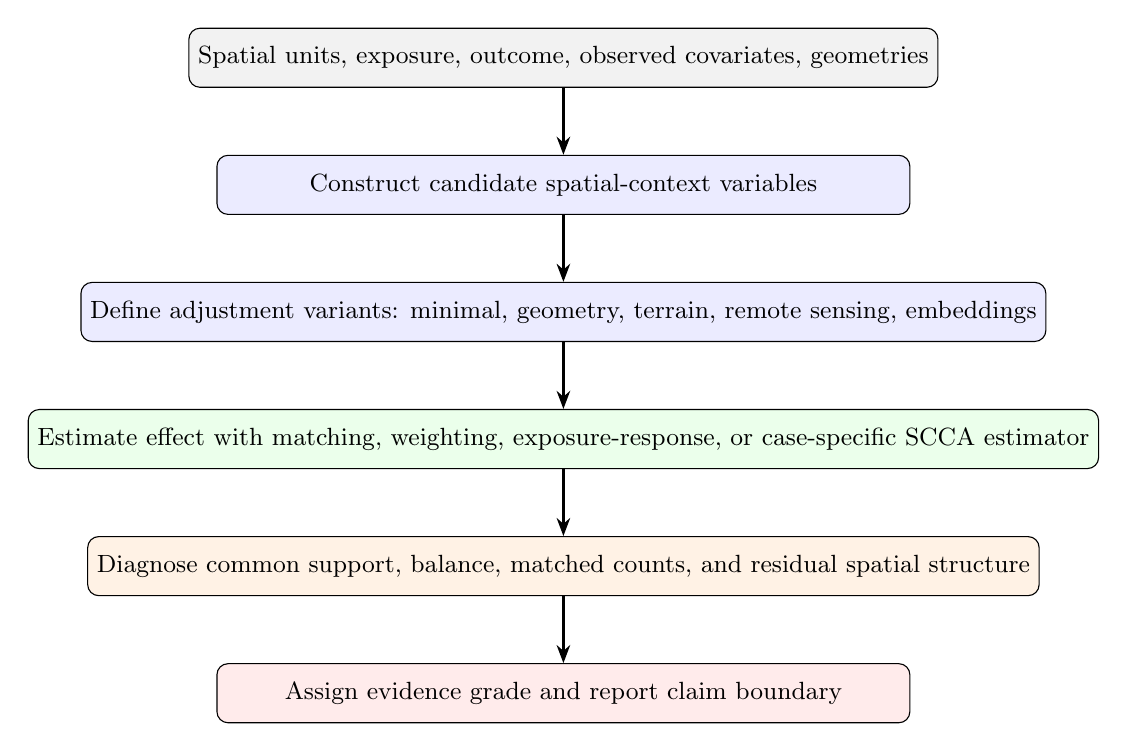
\begin{tikzpicture}[
    node distance=0.85cm,
    box/.style={draw, rounded corners, minimum height=0.75cm, minimum width=8.8cm, align=center, font=\small},
    arr/.style={-{Stealth[length=2.3mm]}, thick}
]
\node[box, fill=gray!10] (input) {Spatial units, exposure, outcome, observed covariates, geometries};
\node[box, fill=blue!8, below=of input] (context) {Construct candidate spatial-context variables};
\node[box, fill=blue!8, below=of context] (variants) {Define adjustment variants: minimal, geometry, terrain, remote sensing, embeddings};
\node[box, fill=green!8, below=of variants] (estimate) {Estimate effect with matching, weighting, exposure-response, or case-specific SCCA estimator};
\node[box, fill=orange!10, below=of estimate] (diagnose) {Diagnose common support, balance, matched counts, and residual spatial structure};
\node[box, fill=red!8, below=of diagnose] (grade) {Assign evidence grade and report claim boundary};
\draw[arr] (input) -- (context);
\draw[arr] (context) -- (variants);
\draw[arr] (variants) -- (estimate);
\draw[arr] (estimate) -- (diagnose);
\draw[arr] (diagnose) -- (grade);
\end{tikzpicture}
}
\caption{SCCA workflow. Spatial context is treated as a candidate adjustment source and must pass support, balance, and robustness diagnostics before it is used to support a causal claim.}
\label{fig:scca_workflow}
\end{figure}

\subsection{Adjustment variants}

For binary treatment, SCCA estimates a propensity score
\begin{equation}
e_i = P(T_i = 1 \mid X_i, C_i)
\end{equation}
for each adjustment variant. Units outside the overlapping propensity-score range are removed. Treated units are matched to controls under a caliper, and standardized mean differences (SMDs) are computed before and after matching:
\begin{equation}
\mathrm{SMD}_k =
\frac{\bar{Z}_{k,T=1} - \bar{Z}_{k,T=0}}
{\sqrt{(s^2_{k,T=1} + s^2_{k,T=0})/2}},
\end{equation}
where $Z_k$ is the $k$th covariate in the adjustment set. A variant is treated as credible only if the maximum post-match absolute SMD is below 0.1 unless a case-specific justification is provided. The estimate is then reported together with matched sample counts and common-support attrition.

\subsection{Robustness diagnostics}

SCCA includes four robustness checks when the data permit them. First, spatial block bootstrap resamples geographic blocks rather than individual units to reduce overconfidence under spatial dependence. Second, placebo exposure definitions test whether the result depends on an arbitrary threshold. Third, placebo or weaker-outcome checks compare the main exposure-outcome relation with less plausible alternatives. Fourth, residual spatial autocorrelation checks whether the matched design still leaves spatially structured residuals. These diagnostics do not prove identification, but they make weak designs visible.

\subsection{Evidence grades}

SCCA assigns one of four evidence grades. \textit{Core support} indicates credible balance or robust synthetic performance plus useful robustness diagnostics. \textit{Bounded support} indicates useful evidence with clear support, scale, balance, or external-validity limits. \textit{Negative ablation} indicates that a tested candidate context source did not improve diagnostics. \textit{Auxiliary only} indicates results that may help interpretation or future work but do not support the main causal adjustment claim.


% ============================================================================
\section{Experiments}
\label{sec:experiments}
% ============================================================================

\subsection{Evidence synthesis design}

The experiments were organized to answer four questions: whether the estimators behave as expected under controlled generators, whether spatial-context adjustment improves a real urban heat analysis, whether SCCA remains useful across distinct geographic case studies, and whether learned geospatial embeddings improve diagnostics over conventional context variables. Table~\ref{tab:evidence_synthesis} summarizes the evidence matrix used to rewrite the manuscript.

\begin{table}[htbp]
\centering
\scriptsize
\setlength{\tabcolsep}{3pt}
\caption{SCCA evidence synthesis. Grades describe claim strength, not statistical significance alone.}
\label{tab:evidence_synthesis}
\begin{tabular}{p{2.0cm}p{1.8cm}p{2.9cm}p{1.7cm}p{2.6cm}}
\toprule
Case & Data type & Key diagnostic & Grade & Manuscript use \\
\midrule
Synthetic benchmark audit & Controlled generators & 48 benchmark rows; 13 robust and 29 fragile rows & Bounded support & Estimator stress test, not real-world validation \\
Chongqing urban heat & Real building and remote-sensing data & Full context ATT = 0.244$^\circ$C; max SMD = 0.061 & Core support & Main real-data SCCA ablation \\
Snow cholera subdistricts & Historical case & Sign stability = 0.985; high exposure-balance correlation = 0.828 & Bounded support & Historical replication with explicit limitation \\
Soho pump proximity & Historical case & Sign stability = 1.000; high exposure-balance correlation = 0.543 & Bounded support & Mechanism-focused historical case \\
County social capital & External county case & Sign stability = 1.000; no downgrade warnings & Core support & Strongest external validation row \\
AlphaEarth ablation & Candidate embedding source & RS/terrain SMD = 0.061; best embedding SMD = 0.268 & Negative ablation & Boundary finding: no clear embedding gain \\
\bottomrule
\end{tabular}
\end{table}

\subsection{Synthetic benchmark audit}

The controlled benchmark used six scenario families: propensity-score matching, difference-in-differences, spatial Granger causality, exposure-response estimation, causal forest heterogeneity, and geographic convergent cross-mapping. Each scenario was run over 30 seeds and stress settings including small samples, noisy outcomes, and severe stress. The audit produced 48 summary rows.

The results were mixed, which is useful for a methods paper because they prevent overclaiming. Difference-in-differences was stable in the baseline setting (RMSE = 0.207 for a true effect of $-8$). Causal forests also recovered the average effect in the baseline setting (RMSE = 1.841 for an effect near 100). Exposure-response estimation remained useful but showed nontrivial bias in some settings. In contrast, the original propensity-score scenario remained biased under the saved generator, and geographic convergent cross-mapping was fragile for direction recovery, with baseline direction accuracy of 0.233 under the standard variant. The audit therefore supports SCCA as a diagnostic wrapper around estimators, not as a guarantee that every estimator works in every spatial setting.

\begin{table}[htbp]
\centering
\scriptsize
\setlength{\tabcolsep}{3pt}
\caption{Selected baseline rows from the synthetic benchmark audit.}
\label{tab:synthetic}
\resizebox{\textwidth}{!}{%
\begin{tabular}{p{2.7cm}p{2.2cm}rrrp{2.8cm}}
\toprule
Scenario & Metric & True value & Mean estimate & RMSE & Interpretation \\
\midrule
Causal forest & ATE & 100.145 & 99.796 & 1.841 & Robust baseline recovery \\
Difference-in-differences & DID & -8.000 & -8.045 & 0.207 & Robust baseline recovery \\
Exposure-response & Range effect & 19.530 & 17.292 & 2.281 & Useful but biased \\
Granger & Direction accuracy & 1.000 & 0.867 & 0.365 & Bounded support \\
PSM & ATT & 15000.000 & 8675.603 & 6569.580 & Fragile generator-estimator alignment \\
GCCM & Direction accuracy & 1.000 & 0.233 & 0.876 & Fragile direction recovery \\
\bottomrule
\end{tabular}
}
\end{table}

\subsection{Chongqing urban heat case}

The main real-data case asked whether high-rise buildings in Chongqing were associated with local summer land surface temperature after spatial-context adjustment. The analysis used a stratified sample of 5,000 buildings from 2021. Treatment was defined as buildings with at least 10 floors. The outcome was summer land surface temperature. Candidate context variables included centroid coordinates, footprint area, Sentinel-2 bands, spectral indices, elevation, and slope.

Table~\ref{tab:chongqing} shows the adjustment variants. The raw mean difference was 0.238$^\circ$C. Several variants achieved credible balance after matching. The full remote-sensing and terrain context specification estimated ATT = 0.244$^\circ$C with 95\% CI [0.148, 0.346] and maximum post-match SMD = 0.061. This replaces the earlier draft's sign-reversal story. The current evidence supports a modest positive association under a balanced SCCA design, not a large negative high-rise cooling effect.

\begin{table}[htbp]
\centering
\small
\caption{Chongqing UHI adjustment variants. Balance pass means maximum post-match SMD $<0.1$.}
\label{tab:chongqing}
\begin{tabular}{lrrrr}
\toprule
Variant & ATT ($^\circ$C) & 95\% CI lower & 95\% CI upper & Max post SMD \\
\midrule
Raw difference & 0.238 & 0.157 & 0.323 & -- \\
Coordinates only & 0.267 & 0.192 & 0.338 & 0.080 \\
Geometry & 0.252 & 0.167 & 0.337 & 0.125 \\
Terrain & 0.303 & 0.220 & 0.381 & 0.104 \\
Sentinel indices & 0.157 & 0.055 & 0.263 & 0.083 \\
Sentinel bands & 0.121 & 0.032 & 0.215 & 0.051 \\
Full RS context & 0.244 & 0.148 & 0.346 & 0.061 \\
PCA context & 0.231 & 0.134 & 0.328 & 0.065 \\
\bottomrule
\end{tabular}
\end{table}

Threshold placebos gave similar positive estimates for the full context specification: 0.222$^\circ$C at an 8-floor threshold, 0.244$^\circ$C at 10 floors, and 0.305$^\circ$C at 12 floors. Residual Moran's $I$ remained significant for both terrain and full context variants (0.112 and 0.102, permutation $p=0.01$), so spatial dependence was reduced but not eliminated. This is why we report the case as credible but bounded by scale mismatch, residual spatial structure, and possible interference.

\subsection{Cross-case SCCA validation}

Three additional cases tested whether the SCCA diagnostic workflow could be used beyond the Chongqing setting. In the South London Snow cholera subdistrict case, the main coefficient was 83.172 and bootstrap sign stability was 0.985, but the maximum exposure-balance correlation was high (0.828), leading to bounded support. In the Soho pump-proximity case, the main coefficient was 1.087 and sign stability was 1.000, but exposure-balance correlation was still high (0.543), again leading to bounded support. In the county social-capital case, the main coefficient was 0.147, sign stability was 1.000, placebo checks were weaker than the main result, and no credibility downgrade warnings were triggered. This case received core support.

These cases are not intended to prove one substantive theory across domains. They test whether SCCA can expose the same design questions across very different geographic datasets: whether the exposure remains distinguishable from background spatial balance variables, whether the estimated direction survives ablation, and whether placebo checks reduce confidence when they should.

\subsection{GeoFM ablation}

The AlphaEarth ablation tested whether learned geospatial embeddings improved adjustment diagnostics in the Chongqing case. They did not. The conventional geometry plus remote-sensing and terrain context variant achieved maximum post-match SMD = 0.061. The best AlphaEarth embedding variant, geometry plus AlphaEarth PCA, had maximum post-match SMD = 0.268. Full 64-dimensional embedding variants also failed the 0.1 balance threshold. Only 199 complete AlphaEarth rows were available in this run, so the finding is a bounded negative diagnostic rather than a general rejection of learned embeddings.

This result is important because it prevents the manuscript from relying on representation hype. In SCCA, a learned embedding is a candidate context source. It becomes useful only when it improves support, balance, robustness, or interpretability in a specific study design. The current ablation supports no stronger claim.


% ============================================================================
\section{Discussion}
\label{sec:discussion}
% ============================================================================

\subsection{What SCCA solves}

SCCA addresses a practical gap in geographic causal analysis: researchers often add spatial variables to an estimator without a transparent account of whether those variables improved the adjustment design. The workflow makes the adjustment set an object of analysis. A reader can see which context sources were tried, which variants passed balance, how many units remained in common support, whether spatial robustness checks were stable, and why the final claim was graded as core, bounded, negative, or auxiliary.

The Chongqing case illustrates the value of this discipline. The most credible current estimate is not the most dramatic estimate. It is the estimate attached to a diagnosed adjustment variant: full remote-sensing and terrain context, acceptable post-match balance, and explicit residual spatial limitations. This is a more defensible contribution than a larger but weakly diagnosed causal story.

\subsection{What SCCA does not solve}

SCCA does not make observational spatial data equivalent to randomized experiments. It cannot adjust for unmeasured confounders that are absent from all candidate context sources. It does not automatically solve interference between neighboring units. It also does not remove the modifiable areal unit problem or scale mismatch between building-level treatments and kilometer-scale remote-sensing outcomes. In the Chongqing case, significant residual Moran's $I$ indicates that spatial structure remains after matching. The correct interpretation is therefore bounded causal evidence under measured context, not definitive identification.

\subsection{Why learned context must be tested}

The GeoFM ablation is a negative but useful result. It shows that adding a high-dimensional learned representation can worsen the diagnosed adjustment design when coverage is limited or when embeddings do not align with treatment assignment and outcome variation. This does not mean such embeddings are useless. It means they should be evaluated as adjustment candidates, not treated as automatically superior confounder controls. Future work should test embedding features on datasets with broader coverage, clearer temporal alignment, and stronger external validation.

\subsection{Auxiliary experiments}

Auxiliary language-model and scenario-simulation experiments were run during development, but they are not used as core SCCA evidence. The language-model validation measured offline graph-recovery behavior and did not estimate treatment effects. The scenario-simulation holdout was an offline proxy in which a persistence baseline outperformed the learned simulator at horizon 1. These results support the decision to keep the present paper focused on SCCA rather than on broader claims about automated causal reasoning or spatial simulation.


% ============================================================================
\section{Conclusions}
\label{sec:conclusions}
% ============================================================================

We presented Spatial Context Causal Adjustment, a diagnostic workflow for geographic observational causal studies. SCCA formalizes spatial context as a candidate adjustment source and requires each adjustment variant to be evaluated through common support, balance, robustness, and evidence-grade diagnostics. Across synthetic benchmarks, a Chongqing urban heat case, historical cholera cases, and a county social-capital validation case, SCCA helped distinguish credible estimates from bounded and fragile designs.

The main empirical result is deliberately bounded. In Chongqing, full remote-sensing and terrain context produced a modest positive high-rise building effect on summer land surface temperature with credible post-match balance. Cross-case analyses showed stable directions but also exposed limitations in historical cholera cases. The AlphaEarth ablation showed no clear gain over conventional remote-sensing and terrain context in the current sample. These findings support SCCA as a reproducible method for auditing spatial causal adjustment, not as a universal solution to spatial confounding.


% ============================================================================
\section*{Declaration of Competing Interest}
% ============================================================================

The authors declare that they have no known competing financial interests or personal relationships that could have appeared to influence the work reported in this paper.

\section*{Data and Code Availability}
% ============================================================================

The repository contains the manuscript source, experiment scripts, generated result tables, diagnostic reports, synthetic generators, and selected sample data needed for reproduction. Remote-sensing and terrain covariates used in the Chongqing case are derived from public geospatial data sources. Raw third-party spatial datasets should be redistributed only where licensing permits. The evidence synthesis used for the revised manuscript is stored in \path{paper/ijgis_submission_20260605/07_results/scca_evidence_synthesis.csv}.


% ============================================================================
\section*{References}
% ============================================================================

\begin{thebibliography}{99}

\bibitem[Angrist and Pischke, 2009]{angrist2009mostly}
Angrist, J.D. and Pischke, J.S., 2009. Mostly Harmless Econometrics: An Empiricist's Companion. Princeton University Press.

\bibitem[Anselin, 1988]{anselin1988spatial}
Anselin, L., 1988. Spatial Econometrics: Methods and Models. Kluwer Academic Publishers.

\bibitem[Athey and Imbens, 2019]{athey2019estimating}
Athey, S. and Imbens, G.W., 2019. Machine Learning Methods That Economists Should Know About. Annual Review of Economics 11, 685--725.

\bibitem[Brown et al., 2025]{brown2025alphaearth}
Brown, C., Kazmierski, M., Pasquarella, V. et al., 2025. AlphaEarth Foundations: An embedding field model for accurate and efficient global mapping from sparse label data. arXiv:2507.22291.

\bibitem[Imbens and Rubin, 2015]{imbens2015causal}
Imbens, G.W. and Rubin, D.B., 2015. Causal Inference for Statistics, Social, and Biomedical Sciences. Cambridge University Press.

\bibitem[Pearl, 2009]{pearl2009causality}
Pearl, J., 2009. Causality: Models, Reasoning, and Inference. 2nd edition. Cambridge University Press.

\bibitem[Rosenbaum and Rubin, 1983]{rosenbaum1983central}
Rosenbaum, P.R. and Rubin, D.B., 1983. The central role of the propensity score in observational studies for causal effects. Biometrika 70(1), 41--55.

\bibitem[Stuart, 2010]{stuart2010matching}
Stuart, E.A., 2010. Matching Methods for Causal Inference: A Review and a Look Forward. Statistical Science 25(1), 1--21.

\bibitem[Sugihara et al., 2012]{sugihara2012detecting}
Sugihara, G. et al., 2012. Detecting Causality in Complex Ecosystems. Science 338(6106), 496--500.

\bibitem[Verburg et al., 2004]{verburg2004lulc}
Verburg, P.H. et al., 2004. Land use change modelling: current practice and research priorities. GeoJournal 61, 309--324.

\end{thebibliography}

\end{document}
